% !TEX root =  ../main_manuscript.tex 

\section{Introduction}
\label{sec:introduction}
Prostate cancer is the second most frequently diagnosed cancer in men worldwide \cite{GlobalCancerStats2012}. The increase in diagnosis of low-grade prostate cancer has been attributed to increase in life expectancy and increase in the number of screening programs \cite{potoskyPSAcancer}. An issue of prostate cancer screening programs is over‐diagnosis. To avoid further over-treatment, patients diagnosed with low-grade prostate cancer are commonly advised to join active surveillance (AS) programs. In AS, serious treatments such as surgery, chemotherapy, or radiotherapy are delayed until cancer progresses. Cancer progression is routinely examined via serum prostate-specific antigen (PSA) levels: a protein biomarker, digital rectal examination (DRE) score: a measure of the size and location of the tumor, medical imaging, and biopsies etc.

While larger values for PSA and/or larger score for DRE, may indicate cancer progression, biopsies are the most reliable prostate cancer progression examination technique used in AS. When a patient's biopsy Gleason grading becomes larger than 6 (definition of cancer progression in this work), AS is stopped and the patient is advised treatment for cancer progression \cite{bokhorst2015compliance}. However, biopsies are invasive, painful, and prone to medical complications \cite{ehdaie2014impact}. Hence, they are conducted intermittently. This leads to a delay in the detection of cancer progression. The delay is equal to the difference between the time of the positive biopsy and the unobserved true time of progression. Hence, the decision of conducting a biopsy requires a fine compromise between the number of biopsies (more is burden) and the delay in detection of progression (less is benefit). 

Currently there is no consensus on the frequency of biopsies in AS \cite{loeb2014heterogeneity}. Majority of the programs focus on minimizing only the delay, by scheduling biopsies annually. Annual biopsies, and other heuristic schedules\cite{inoue2018comparative} which do not account for the difference in cancer progression speeds of patients, may work well for patients who progress fast or for patients for whom the initial biopsy Gleason score was incorrect. However, for slowly progressing patients (majority of AS patients) many unnecessary burdensome biopsies are scheduled. To mediate the burden between fast and slow progressing patients, the world's largest AS program, Prostate Cancer Research International Active Surveillance (PRIAS) \cite{bul2013active}, schedules annual biopsies only for patients with a small PSA doubling time\cite{bokhorst2015compliance}. For everyone else, PRIAS schedules biopsies at following fixed follow-up times: year 1, 4, 7, and 10, and every 5 years thereafter. Despite this effort, in PRIAS over a period of 10 years a patient may get scheduled for 4 to 10 biopsies. Consequently, patients may not always comply with the schedule \cite{bokhorst2015compliance}. This can lead to the original problem of delayed detection of prostate cancer progression, and reduce the effectiveness of AS.
 
\begin{figure}[!htb]
\captionsetup{justification=justified}
\centerline{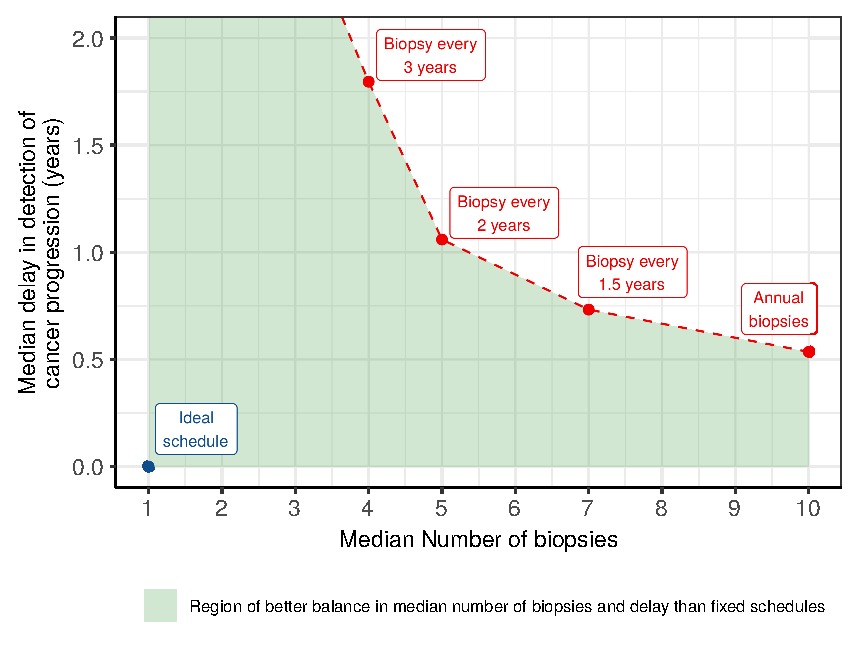
\includegraphics[width=\columnwidth]{images/better_balance_intro.eps}}
\caption{Median number of biopsies scheduled by various fixed scheduling approaches (in red) in practice (over a follow-up of 10 years), and the corresponding median delay in detection of cancer progression. An ideal schedule (in blue) will schedule only 1 biopsy, exactly at the true time of cancer progression. We intend to better balance the number of biopsies and the delay, than in practice currently, using personalized decision making for biopsies.}
\label{fig:better_balance_intro}
\end{figure}

This article is motivated by the need to better balance the number of biopsies and the delay in detection of prostate cancer progression, than in practice currently (see Figure~\ref{fig:better_balance_intro}). We intend to achieve this by personalizing the decision of conducting biopsies at follow-up visits. To this end, we utilize the data of the patients of the PRIAS study (see Figure~\ref{fig:obsDataPlot_2340}). Personalized decision making has received much interest in the literature, especially for screening of various cancers by utilizing Markov decision process models \cite{ayer2012or, akhavan2017markov,erenay2014optimizing}. In case of prostate cancer, Zhang~et~al.\cite{zhang2012optimization} personalized the decision of biopsies using these models, to avoid over-diagnosis during screening. Their model used baseline patient characteristics as well as the latest PSA level (discretized) of the patient.

\begin{figure}[!htb]
\captionsetup{justification=justified}
\centerline{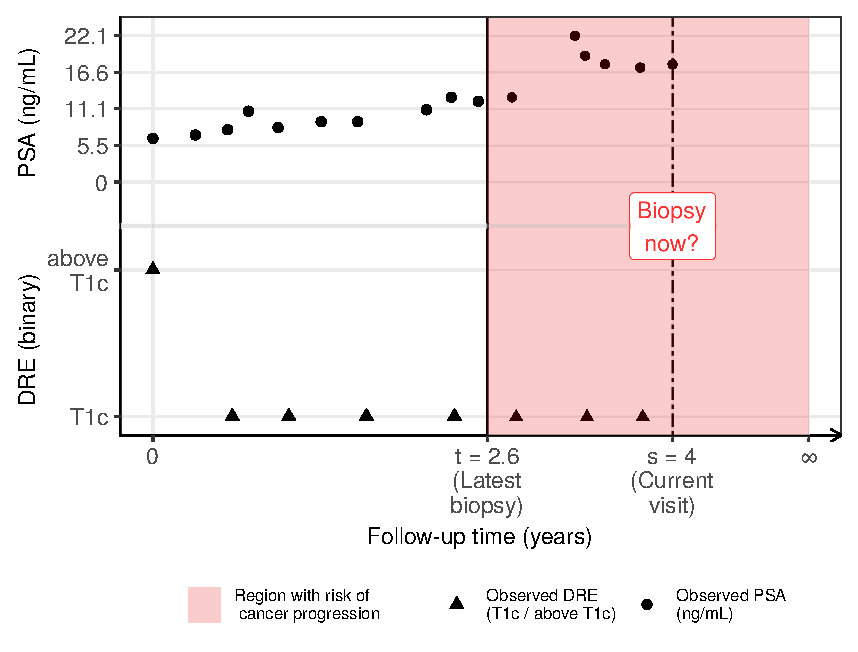
\includegraphics[width=\columnwidth]{images/obsDataPlot_2340.eps}}
\caption{\textbf{Illustration of the decision making problem}: Available data of a patient, who had his latest (negative) biopsy at $t=2.6$ years. The shaded region shows the time period in which the patient is at the risk of cancer progression. His current follow-up visit is at $s=4$ years. Using the entire history of DRE $\mathcal{Y}_{dj}(s)$ and PSA $\mathcal{Y}_{pj}(s)$ measurements up to current visit time $s$, and the time of latest biopsy $t$, we intend to make a decision on scheduling a biopsy at $s$.}
\label{fig:obsDataPlot_2340}
\end{figure}

In comparison to the work referenced above, we do not base the decision of biopsy only on the latest PSA level of a patient, but instead we use the entire history, of DRE scores, PSA levels and the unobserved rate of change of PSA (PSA velocity), and results of the latest biopsy. To this end, we employ joint models for time-to-event and longitudinal data \cite{tsiatis2004joint,rizopoulos2012joint}. Joint models utilize patient-specific random effects \cite{laird1982random} to model the observed data, and hence they are inherently personalized. Using joint models we first obtain a full specification of the joint distribution of the time of cancer progression, and PSA and DRE measurements. We then use it separately for each patient at each follow-up visit to develop a cancer progression risk profile, based on their observed data. If the risk is higher than a certain threshold our method schedules a biopsy at the same follow-up visit. Since there is no clear consensus on choice of risk thresholds, we not only use fixed thresholds suggested by urologists, but also present a methodology to automate the choice of thresholds. 

In order to compare the personalized approach, with the in-practice annual and PRIAS schedules, we conduct an extensive simulation study. For a realistic comparison, we simulate a replica of the population of the PRIAS patients, using the joint model fitted to the PRIAS dataset.

The rest of the article is structured as follows: The details of the joint modeling framework and biopsy decision making methodology are presented in the \hyperref[sec:methods]{Methods} section. The details of the simulation study and the corresponding results are presented in \hyperref[sec:methods]{Methods} and \hyperref[sec:results]{Results} sections, respectively.